\documentclass[11pt,a4paper]{article}
\usepackage{fdicpaper}
\hypersetup{pdftitle={Bank-Failure Early Warning Using FDIC Data},pdfauthor={Nguyen Le Nam Khanh}}
\begin{document}
\begin{titlepage}
\centering
\vspace*{7mm}
{\fontsize{18}{22}\selectfont\bfseries Bank-Failure Early Warning\\Using FDIC Data\par}
\vspace{3mm}
{\normalsize Data Engineering, Temporal Validation and Review Costs\par}
\vspace{7mm}
{\microtypesetup{protrusion=false}\fontencoding{T5}\fontfamily{qtm}\selectfont\large Nguyễn Lê Nam Khánh\par}
\vspace{2mm}
{\normalsize\itshape National Economics University, Hanoi, Vietnam\par}
\vspace{3mm}
{\normalsize Student ID: 11230976\par}
{\small BFT65B -- Big Data Analytics in Finance\par}
{\normalsize 15 November 2026\par}
\vspace{6mm}
{\bfseries Abstract\par}
\vspace{2mm}
\begin{minipage}{.92\textwidth}
\small\setstretch{1.08}\setlength{\parindent}{0pt}
This project constructed a financial reporting pipeline from FDIC data covering 1984Q1--2026Q2. The acquired sample contains 1,682,616 reports across 170 quarters. Original responses were retained alongside typed Parquet tables, with financial reporting exceptions documented before feature construction. For an identical seven-column projection, Parquet reduced storage from 68.56 to 18.05 MB. The matched join and aggregation took a median 0.073 seconds in Polars and 0.569 seconds in pandas, while a local Spark implementation reproduced the aggregate results. Model development used 64 chronological validation folds. On the final 2013Q1--2025Q2 holdout, the selected iterative random forest attained mean annual average precision of 0.251 and detected 68 of 78 failures at an illustrative quarterly alert share of 3.53\%, with precision of 2.23\%. A seven-feature forest achieved higher mean annual average precision of 0.310. Review-cost scenarios quantified the associated workload under assumptions about review effort and missed-event severity. The results support a local columnar workflow for this panel and identify the operational measurements needed to evaluate its use in supervision.
\end{minipage}\par
\vspace{5mm}
\begin{minipage}{\textwidth}
\small\setstretch{1.0}\setlength{\parindent}{0pt}
\textit{Keywords:} bank failure; financial data engineering; temporal validation; rare events; review costs.
\par\vspace{4mm}
\textbf{Data and evaluation scope}\par\vspace{2mm}
\begin{tabularx}{\linewidth}{@{}p{.24\linewidth}X@{}}
\toprule
Acquisition & FDIC BankFind public API; downloaded 6 November 2026.\\
Source coverage & Financials 1984Q1--2026Q2: 1,682,616 rows, 170 quarters, 87 fields; Failures: 4,117 records; Institutions: 27,835 records.\\
Development & Final training sample, prediction quarters 1984Q2--2011Q4: 1,306,763 rows and 2,729 represented failures; validation 1996--2011: 594,873 rows and 514 events per primary scheme.\\
Holdout & Prediction quarters 2013Q1--2025Q2, after the 2012 gap: 273,863 evaluable rows and 78 failures; labels complete through 2026Q2.\\
Repository & \url{https://github.com/khanhnlmneuron6-hue/fdic-bank-failure-risk-analytics}\\
\bottomrule
\end{tabularx}
\end{minipage}
\end{titlepage}
\section*{Introduction}
\addcontentsline{toc}{section}{Introduction}
Bank supervision requires financial reports that remain comparable as institutions merge, reporting conventions change and economic conditions deteriorate. This project uses US bank data to examine how a central-bank supervision team could construct such a panel and use it to rank institutions for further review. The emphasis is on data preparation and processing, with bank-failure prediction providing an application through which to evaluate the resulting dataset.

Earlier studies support the use of accounting information for this purpose. Petropoulos et al. found that random forests performed well in comparisons of models for US bank insolvency, including evaluation on later periods \citep{petropoulos}. Their outcome includes assistance transactions as well as failures. The historical evidence in Correia, Luck and Verner links failures to deteriorating fundamentals and funding structures \citep{failingbanks}. These findings inform the feature families considered here, while the present analysis defines its outcome as the first qualifying failure of an insured institution.

The pipeline covers more than four decades of FDIC reports and was evaluated through chronological validation and a final holdout. Its selected model detected 68 of 78 holdout failures at an illustrative quarterly alert share of 3.53\%, although a simpler reference achieved higher average precision.

\section{Acquisition and storage}
\subsection{Source coverage and completeness}
The data were downloaded from the FDIC BankFind public API on 6 November 2026 \citep{fdicapi}. Financials contains 1,682,616 reports spanning 170 quarters from 1984Q1 to 2026Q2, with 87 fields covering financial values, institutional identifiers and audit information. The accompanying Failures and Institutions tables contain 4,117 and 27,835 records, respectively. CERT identifies institutions across the three sources.

The downloader requested a fixed field list and retrieved successive pages within each quarter, retrying interrupted requests. It retained the original responses as compressed JSON and recorded the requested fields, API totals and file hashes in acquisition manifests. All 170 quarterly row counts matched the totals recorded at download. These checks refer to the retained November snapshot, which may differ from later downloads as the FDIC revises its data.

\subsection{Storage design and measured compression}
Raw response files were kept unchanged so that derived values could be traced to their inputs. Analytical tables were stored as typed Parquet files partitioned by report quarter, allowing transformations to select the required dates and columns \citep{parquet,polars}. The acquisition manifests also support resumption by checking that completed partitions have the expected fields and hashes.

\begin{figure}[!htbp]
\centering
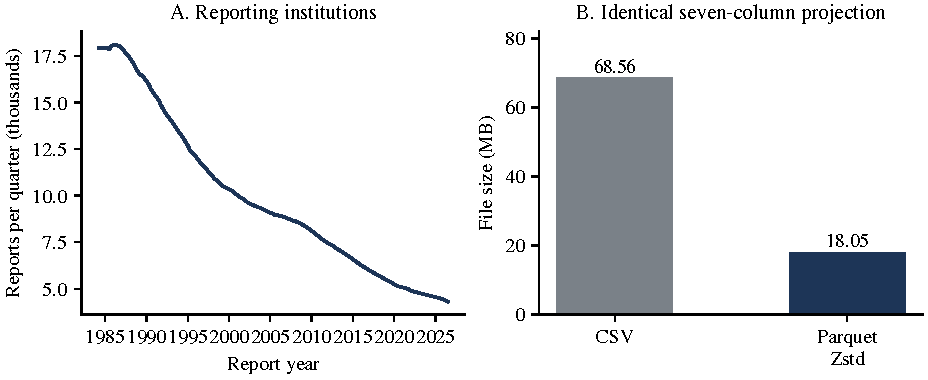
\includegraphics[width=\linewidth]{../figures/paper/data_and_storage.pdf}
\caption{Reporting coverage and storage requirements.}
\label{fig:1}
\papernotes{Panel A counts financial reports by quarter. Panel B uses an identical projection of 1,350,892 rows and seven columns for 1984Q1-2011Q3. Sizes use decimal MB. Sources: \evidence{acquisition_completeness.csv} and \evidence{storage_sizes.json}.}
\end{figure}
For the matched seven-column projection, CSV required 68.56 MB and Parquet with Zstd compression required 18.05 MB. The resulting size ratio was 3.80. This measurement supports the choice of Parquet for repeated analytical scans of the panel. The processing comparison in Section 3 uses the same projection.

\section{Data quality and panel construction}
\subsection{Financial reporting exceptions}
The quality checks distinguished unusual financial conditions from reporting problems. Negative equity and losses were retained as potential indicators of distress, while negative stock values and inconsistent accounting components were flagged for investigation. A ratio with a missing or nonpositive denominator remained undefined. Genuine zero balances, such as an absence of borrowing, were preserved.

\begin{table}[!htbp]
\centering
\begin{threeparttable}
\caption{Selected exceptions identified by the automated quality checks.}
\label{tab:1}
\small\setstretch{1.0}\setlength{\tabcolsep}{4pt}\renewcommand{\arraystretch}{1.15}
\begin{tabular}{@{}L{\dimexpr 0.34402\linewidth-2\tabcolsep\relax}R{\dimexpr 0.16548\linewidth-2\tabcolsep\relax}L{\dimexpr 0.49051\linewidth-2\tabcolsep\relax}@{}}
\toprule
\textbf{Condition} & \textbf{Flagged rows} & \textbf{Treatment} \\
\midrule
Negative equity & 14,899 & Retain as an economically meaningful condition. \\
Liabilities above assets & 14,819 & Flag and reconcile with equity and other balance-sheet items. \\
Suspected restart of YTD flows & 5,510 & Review the affected income sequence. \\
Negative stock value & 2,260 & Investigate and isolate affected derived values where required. \\
Nonpositive gross loans & 13,362 & Leave ratios using that denominator undefined. \\
Nonpositive deposits & 8,762 & Leave the loan-to-deposit ratio undefined. \\
\bottomrule
\end{tabular}
\begin{tablenotes}[flushleft]
\footnotesize\setstretch{1.0}
\item \textit{Notes.} Scope: 1,350,892 raw reports, 1984Q1-2011Q3. Flags can overlap within a row. Flagged observations were reviewed under the financial rules described in the text. Source: \evidence{source_quality_flags.csv}.
\end{tablenotes}
\end{threeparttable}
\end{table}
Income reporting required a separate treatment because Call Report income schedules record amounts accumulated since the start of the calendar year \citep[Schedule RI-1]{ffiec}. The pipeline used a reported quarterly counterpart where available and otherwise calculated differences between consecutive reports for the same CERT. Trailing-twelve-month (TTM) measures required four consecutive calendar quarters.

A decline across several YTD income items was treated as a possible change in the accounting basis. Affected TTM windows were set to missing under the rule identified as Y1 in the implementation. Limited accounting identities recovered selected historical values when consistency checks were satisfied. Subsequent successor relationships were reserved for audit evidence, so recovery of a predictor depended on information allowed by the feature construction rules.

The rules also isolated an ambiguous real-estate decomposition in historical thrift reports. Each adjustment was recorded against the affected derived cell, with the original value retained. This record distinguishes missing history, undefined ratios and suspected reporting problems before imputation. Numerical parity checks confirmed that the revised feature builder reproduced the approved research representation within the specified tolerance.

\subsection{Outcome definition and institution exits}
The binary target records whether institution i experiences its first qualifying failure during the four quarters following prediction date t. \textit{T}\textsubscript{i} denotes the date of that failure. Mergers and assistance transactions were classified separately.

\begin{equation}
y_{i,t}=\mathbf{1}\!\left\{t<T_i\leq t+4\ \text{quarters}\right\},
\label{eq:1}
\end{equation}
The modelling population excluded observations after an institution had exited and observations outside the eligible insured population. Incomplete outcome horizons and uncertain exits were censored under the recorded population rules. Current institution metadata helped classify outcomes but was excluded from the predictor matrix. Because several reporting quarters can precede the same failure, the evaluation tracks both positive rows and unique failure events.

\subsection{Information timing and analytical samples}
A financial report for quarter r was assumed available at the end of quarter r + 1. Features were joined to the corresponding prediction date using CERT and exact calendar quarters. This one-quarter lag approximates publication availability because historical release timestamps are unavailable in the retained snapshot.

The final training sample ended at 2011Q4, with its outcomes complete by 31 December 2012. The year 2012 provided a gap before the holdout began in 2013Q1. The holdout ended at 2025Q2, allowing its one-year outcomes to be observed through 2026Q2. Table 2 reports the observations and failure events included at each stage.

\begin{table}[!htbp]
\centering
\begin{threeparttable}
\caption{Acquisition records and analytical populations.}
\label{tab:2}
\small\setstretch{1.0}\setlength{\tabcolsep}{4pt}\renewcommand{\arraystretch}{1.15}
\begin{tabular}{@{}L{\dimexpr 0.48833\linewidth-2\tabcolsep\relax}R{\dimexpr 0.17419\linewidth-2\tabcolsep\relax}R{\dimexpr 0.16983\linewidth-2\tabcolsep\relax}R{\dimexpr 0.16765\linewidth-2\tabcolsep\relax}@{}}
\toprule
\textbf{Population} & \textbf{Rows} & \textbf{Positive rows} & \textbf{Failure events} \\
\midrule
\addlinespace[3pt]\multicolumn{4}{@{}l}{\textit{Panel A. Source records}} \\
\addlinespace[2pt]
Financials, 1984Q1-2026Q2 & 1,682,616 & - & - \\
Failures source & 4,117 & - & Source records \\
Institutions source & 27,835 & - & - \\
\addlinespace[3pt]\multicolumn{4}{@{}l}{\textit{Panel B. Analytical samples}} \\
\addlinespace[2pt]
Final training, 1984Q2-2011Q4 & 1,306,763 & 10,564 & 2,729 \\
Validation, 1996-2011 & 594,873 & 1,981 & 514 \\
Initial holdout keys & 280,267 & - & - \\
Less: unlabelled or ineligible & (6,404) & - & - \\
Evaluable holdout, 2013Q1-2025Q2 & 273,863 & 257 & 78 \\
\bottomrule
\end{tabular}
\begin{tablenotes}[flushleft]
\footnotesize\setstretch{1.0}
\item \textit{Notes.} Validation counts are per primary scheme. The holdout population follows the registered eligibility and nonnull-label criteria. Sources: \evidence{acquisition_summary.json}, \evidence{final_fit_manifest.json}, \evidence{B3_dev_operating_metrics.csv}, \evidence{test_population_reconciliation.json} and \evidence{test_metrics.csv}.
\end{tablenotes}
\end{threeparttable}
\end{table}
\section{Scalable processing}
\subsection{Comparable transformations in pandas and Polars}
The processing comparison applied the same scan, exact-quarter self-join, financial ratios and quarterly aggregation to the seven-column projection. CSV types were supplied explicitly. Each pandas and Polars operation was repeated three times under a warm operating-system cache, and numerical equivalence was checked before execution times were compared.

\begin{table}[!htbp]
\centering
\begin{threeparttable}
\caption{Execution times for the matched local workload.}
\label{tab:3}
\small\setstretch{1.0}\setlength{\tabcolsep}{4pt}\renewcommand{\arraystretch}{1.15}
\begin{tabular}{@{}L{\dimexpr 0.52099\linewidth-2\tabcolsep\relax}R{\dimexpr 0.13064\linewidth-2\tabcolsep\relax}L{\dimexpr 0.34837\linewidth-2\tabcolsep\relax}@{}}
\toprule
\textbf{Operation} & \textbf{Seconds} & \textbf{Measurement} \\
\midrule
pandas: CSV scan & 0.3064 & Median of three repetitions \\
pandas: Parquet scan & 0.0577 & Median of three repetitions \\
Polars: Parquet scan & 0.0223 & Median of three repetitions \\
Polars: two-column projection & 0.0055 & Median of three repetitions \\
Polars: join, ratios and aggregate & 0.0731 & Median of three repetitions \\
pandas: join, ratios and aggregate & 0.5689 & Median of three repetitions \\
Spark: local query & 2.9428 & One action, startup excluded \\
\bottomrule
\end{tabular}
\begin{tablenotes}[flushleft]
\footnotesize\setstretch{1.0}
\item \textit{Notes.} The projection comprises CERT, REPDTE, ASSET, EQ, LNLSGR, NCLNLS and NETINC. Measurements used a macOS arm64 laptop with 10 logical CPUs. The Spark query ran in local[2] mode. Its timing is reported separately from the repeated pandas/Polars benchmark. Sources: \evidence{storage_processing_benchmarks.csv}, \evidence{storage_sizes.json} and \evidence{spark_mllib_demo.json}.
\end{tablenotes}
\end{threeparttable}
\end{table}
Polars completed the join, ratios and aggregation in a median 0.073 seconds, compared with 0.569 seconds for pandas. Parquet scans were also faster than the CSV scan in this workload. The optimized Polars plan reused the scan through a cache and projected the right-hand join input to the required keys and income column. The query was collected after the transformations and aggregation \citep{polars}. Exact calendar keys ensured that a missing quarter remained a gap rather than becoming the previous available row.

\subsection{Spark results and implications for scaling}
The Spark implementation reproduced the benchmark transformations and agreed with pandas and Polars on all reported aggregate columns. The maximum floating-point difference was approximately 5 \(\times\) 10\textsuperscript{-14}. Its query action took 2.943 seconds after startup. The saved physical plan includes an adaptive execution plan, join stages and an ordered final result, providing a basis for examining partitioning and exchanges \citep{spark}.

The acquisition and panel-processing tasks completed on the laptop. For this workload, local Polars avoided the scheduling overhead evident in the Spark demonstration. A cluster would become relevant for wider transaction joins, concurrent analytical jobs or workloads whose intermediate results exceed local memory. That decision would require measurements of memory consumption and shuffle volume at the intended scale, since the present timing comparison covers a local execution only.

\section{Feature construction and preprocessing}
\subsection{Financial representation}
The feature pool comprised 21 economic groups constructed from the 87 source fields. Capital adequacy and asset quality describe loss absorption and impaired exposures, while earnings, funding ratios and portfolio concentrations provide further measures of financial condition \citep{petropoulos,failingbanks}. Groups combined current levels, TTM income measures and changes over four quarters.

\begin{table}[!htbp]
\centering
\begin{threeparttable}
\caption{Feature families and construction rules.}
\label{tab:4}
\small\setstretch{1.0}\setlength{\tabcolsep}{4pt}\renewcommand{\arraystretch}{1.15}
\begin{tabular}{@{}L{\dimexpr 0.27217\linewidth-2\tabcolsep\relax}L{\dimexpr 0.72783\linewidth-2\tabcolsep\relax}@{}}
\toprule
\textbf{Family} & \textbf{Representation} \\
\midrule
Capital and asset quality & Equity/assets, noncurrent loans, other real estate (ORE)/assets and nonperforming assets (NPA)/assets. \\
Earnings and provisions & Return on assets (ROA), net interest margin (NIM) and provisions based on validated quarterly flows. \\
Concentration and liquidity & Four real-estate shares, cash/assets and securities/assets. \\
Changes over four quarters & Differences matched by CERT and the exact quarter four periods earlier. \\
Loss-buffer measures & Texas proxy, nonpositive-buffer indicator, buffer gap/assets and uncovered noncurrent loans/assets. \\
\bottomrule
\end{tabular}
\begin{tablenotes}[flushleft]
\footnotesize\setstretch{1.0}
\item \textit{Notes.} Exact formulas and column order are recorded in \evidence{final_feature_contracts.csv}. Financial amounts use thousands of USD and ratios use percent. Unavailable histories remain missing until preprocessing.
\end{tablenotes}
\end{threeparttable}
\end{table}
Forward selection used histogram gradient boosting (HGB) to evaluate economic groups within each training window. After the modelling procedure was selected, the selector was fitted again on the complete development sample, retaining 12 groups with 20 columns. Four additional loss-buffer measures brought the final candidate to 24 predictors. This candidate is labelled B3 in the experiment records and in the result tables.

The additional measures describe impaired assets relative to tangible capital and loan-loss reserves. The Texas proxy uses noncurrent loans plus ORE in its numerator and equity less intangibles plus reserves in its denominator. A separate indicator records a nonpositive denominator, while the gap and uncovered-loan measures express shortfalls relative to total assets. These features were introduced after earlier development comparisons, which is relevant to the selection uncertainty discussed in Section 6.

\subsection{Preprocessing within training samples}
For each fit, the pipeline estimated domain-specific clipping bounds from the training sample and then fitted median imputation to the same observations. Signed financial quantities and changes retained their permitted signs, with special handling for sparse positive tails. The capper implementation is named ContractCapperV4 in the source code. Logistic regression additionally used standardization fitted on the training sample. A fit was stopped if any predictor had entirely missing training values.

A separate record retained the reasons for missing values after imputation. These reasons were not supplied to the model as predictors. Median imputation without missingness indicators can therefore make an imputed value indistinguishable from an observed value at the median. Earlier comparisons examined alternative clipping and indicator specifications, and the final model retained the representation selected during development. Their results apply to the tested specifications and evaluation periods.

\section{Modelling and validation}
\subsection{Chronological validation and evaluation metrics}
Validation covered 16 years from 1996 to 2011 under fixed-origin, expanding, rolling-five-year and rolling-ten-year training schemes. The schedule therefore comprised 64 folds but only 49 distinct training windows, allowing identical training samples to share a fit. Feature selection and preprocessing were repeated within each training window, with label maturity and a four-quarter gap enforced.

The primary comparison used the fixed-origin and rolling-five-year schemes. Ranking was assessed with non-interpolated average precision (AP), computed from the precision-recall curve \citep{sklearnap}. Mean annual AP gave equal weight to years containing positive rows, excluding 2005 from development because it had no positives. Pooled AP was computed over all observations together. In equation (2), \textit{R}\textsubscript{k} and \textit{P}\textsubscript{k} denote recall and precision at successive score thresholds, and the set of years containing positives is \textit{Y}\textsubscript{+}.

\begin{equation}
\operatorname{AP}=\sum_k(R_k-R_{k-1})P_k,\qquad \overline{\operatorname{AP}}_{\mathrm{year}}=\frac{1}{|\mathcal{Y}_{+}|}\sum_{y\in\mathcal{Y}_{+}}\operatorname{AP}_y.
\label{eq:2}
\end{equation}
Precision and row recall assessed the quarterly alerts, while event recall measured the proportion of unique failures preceded by at least one eligible positive-quarter alert. Lead time and alert volume described the timing and workload of detection. These quantities are useful alongside AP when failures are rare \citep{saito}.

Development selection combined mean annual AP and event recall at a reference 5\% alert share across the two primary schemes. The minimax relative-regret criterion, recorded as D43 in the research documentation, favored B3. The 5\% share represented an evaluation preference. The subsequent cost analysis selected the final illustrative alert share separately. Repeated inspection and extension of the candidate set can introduce selection optimism despite chronological splitting \citep{cawley}.

\subsection{Models and development results}
The selected model used an iterative random forest (iRF), which reweights feature sampling across successive forests \citep{basu}. It contained 50 trees with maximum depth 6 and a minimum leaf size of 50, fitted over three reweighting iterations. Bootstraps used for interaction discovery were disabled in the predictive implementation \citep{imodels}. This specification was held fixed in the reported iRF comparisons.

The controls comprised iRF and logistic regression fitted to seven core features. These were equity/assets, noncurrent loans, reserves/loans, ROA, loans/deposits, borrowing/assets and log assets. Development experiments also evaluated an expanded feature pool and XGBoost classifier and ranking models, with tuning conducted inside the corresponding training samples.

\begin{figure}[!htbp]
\centering
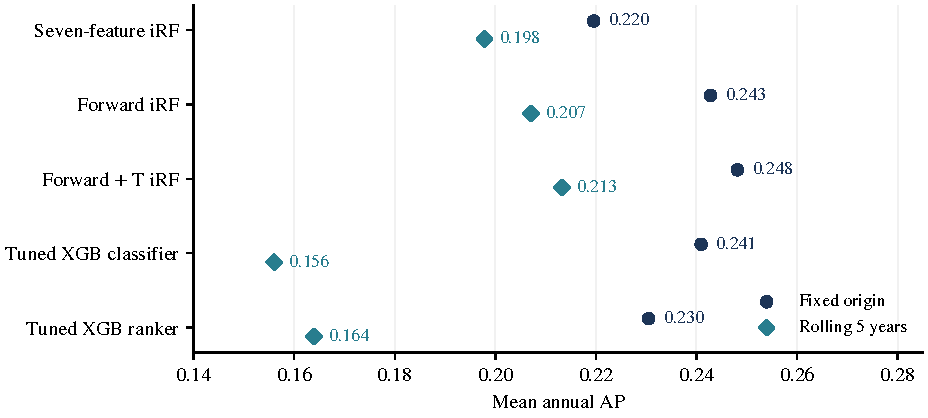
\includegraphics[width=\linewidth]{../figures/paper/model_comparison.pdf}
\caption{Model comparison under the two primary validation schemes.}
\label{fig:2}
\papernotes{Points report mean annual AP. The forward + T iRF specification is B3, with T denoting its four loss-buffer features. XGBoost used the seven core features plus T. Comparisons used the full training samples. Source: \evidence{v65_branch_scores.csv}.}
\end{figure}
B3 increased mean annual AP from 0.243 to 0.248 under fixed-origin validation and from 0.207 to 0.213 under rolling-five-year validation relative to the forward-selected forest without the additional loss-buffer measures. Selection from the expanded pool did not improve the two primary comparisons. Tuned XGBoost classifier and ranking models remained below the iRF candidates, with larger shortfalls under rolling-five-year training. Supplementary selector and model comparisons appear in Appendix A.

\subsection{Variation across economic periods}
\begin{figure}[!htbp]
\centering
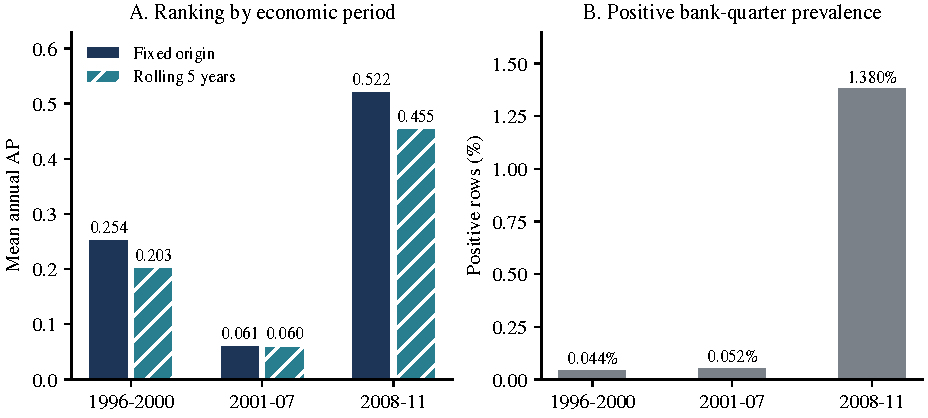
\includegraphics[width=\linewidth]{../figures/paper/period_ranking.pdf}
\caption{B3 ranking performance and failure prevalence by period.}
\label{fig:3}
\papernotes{Panel A reports mean annual AP. Panel B reports positive-row prevalence for the fixed-origin sample in each period. Source: \evidence{v62_period.csv}.}
\end{figure}
Mean annual AP for B3 was approximately 0.060 during 2001-2007, compared with 0.522 during 2008-2011 under fixed-origin validation. Positive-row prevalence also increased from 0.052\% to 1.380\% between these periods. Since AP depends on the class distribution, the observed gap reflects a comparison of different economic and event environments as well as model performance \citep{saito}.

The prediction diagnostics found weaker ranking among observations nine to twelve months before failure and limited precision near the top of the list. A failure could still count as detected if the bank received an alert in a later positive quarter. High event recall can thus coexist with weaker early detection. Strictly monotone probability calibration preserves score ordering and would not address that ranking limitation by itself.

\subsection{Alert policy and cost assumptions}
Each eligible institution received a risk score, and the alert policy selected a quarterly share q for an offsite desk review. The cost calculation distinguished new reviews from reviews repeated in consecutive quarters. A nonalerted or missing quarter started a new review when an alert next appeared, and the holdout review history began without prior alerts.

Equation (3) combines review effort with the severity of missed failure events. Here c is the hourly cost in 2012 dollars, h is the time required for a first review, and \(\rho\) is repeat effort relative to a first review. \textit{S}\textsubscript{missed} sums missed-event severity in thousands of 2012 dollars, with each missed event counted once. The weight \(\alpha\) specifies the decision scenario \citep{sarlin,elkan}.

\begin{equation}
L(q)=\frac{ch}{1000}\left[N_{\mathrm{new}}(q)+\rho N_{\mathrm{repeat}}(q)\right]+\alpha S_{\mathrm{missed}}(q).
\label{eq:3}
\end{equation}
\begin{table}[!htbp]
\centering
\begin{threeparttable}
\caption{Inputs to the review-cost scenarios.}
\label{tab:5}
\small\setstretch{1.0}\setlength{\tabcolsep}{4pt}\renewcommand{\arraystretch}{1.15}
\begin{tabular}{@{}L{\dimexpr 0.21991\linewidth-2\tabcolsep\relax}L{\dimexpr 0.35490\linewidth-2\tabcolsep\relax}L{\dimexpr 0.42519\linewidth-2\tabcolsep\relax}@{}}
\toprule
\textbf{Input} & \textbf{Source or interpretation} & \textbf{Treatment} \\
\midrule
USD 110 per hour & Historical OCC fee \citep{occ} & Proxy for hourly review cost. \\
4 or 12 hours & FDIC OIG interviews \citep{oig2019} & Alternative first-review scenarios. \\
Repeat effort \(\rho\) & Unobserved workflow quantity & Values 0.25, 0.5 and 1, with 0.5 in the primary case. \\
Severity weight \(\alpha\) & Decision preference and intervention uncertainty & Grid from 0 to 0.1, with 0.001 in the primary case. \\
FDIC COST and CPI & Estimated fund loss and price conversion \citep{fdicapi,cpi,fdicloss} & 2012 price basis, preserving zero and using a development-cohort median for missing severity. \\
Capacity and escalation & Staffing assumptions and examination benchmarks \citep{oig2012} & Separate workload sensitivity calculations. \\
\bottomrule
\end{tabular}
\begin{tablenotes}[flushleft]
\footnotesize\setstretch{1.0}
\item \textit{Notes.} COST measures estimated loss to the deposit insurance fund. Revised COST and CPI are used as retrospective severity weights. Scenario definitions are recorded in \evidence{docs/cost_policy.json}.
\end{tablenotes}
\end{threeparttable}
\end{table}
The hourly proxy follows the OCC fee for special examinations and investigations \citep[p. 4]{occ}. The 4- and 12-hour cases reflect heterogeneous review times reported in interviews with 32 case managers \citep[p. 11]{oig2019}. Actual staff cost, repeat effort and intervention effectiveness were not estimated from the bank panel. The reported loss is consequently conditional on these assumptions.

\begin{figure}[!htbp]
\centering
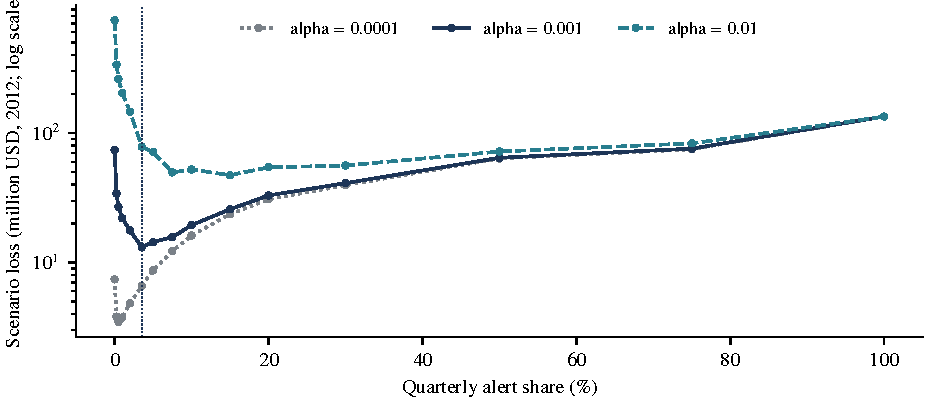
\includegraphics[width=\linewidth]{../figures/paper/cost_sensitivity.pdf}
\caption{Sensitivity of development loss to the alert share and severity weight.}
\label{fig:4}
\papernotes{B3 fixed-origin predictions with c = USD 110/hour, h = 4 and \(\rho\) = 0.5. The vertical line marks q = 3.53\%, selected for \(\alpha\) = 0.001 from the specified finite grid. Sources: \evidence{cost_scenarios.csv} and \evidence{docs/cost_policy.json}.}
\end{figure}
Under the primary scenario, the development loss was minimized at q = 3.53\%. This produced 20,849 alerts, comprising 5,850 new reviews and 14,999 repeats, and detected 473 of 514 failures. Estimated review effort totaled 53,398 hours and peaked at 1,664 hours in one quarter. Review cost was USD 5.874 million and total scenario loss was USD 13.108 million in 2012 prices.

The selected share was fixed before the holdout evaluation. Rolling-five-year outcomes and alternative review durations were retained as sensitivity cases. Capacity calculations applied assumptions about productive hours and staff allocation, while escalation scenarios used examination workloads of 335-1,820 hours for banks with assets up to USD 1 billion \citep[Table 3]{oig2012}. These quantities describe different supervisory activities and require local workflow evidence before operational use.

\subsection{Final holdout evaluation}
B3 and the two seven-feature controls were fitted on the complete development sample after their specifications had been selected. The features and alert share were fixed before the 2013Q1-2025Q2 holdout was scored. Each model received one scoring pass on the 273,863 eligible observations, whose positive rate was 0.094\%. The comparisons below were calculated from those saved predictions.

\begin{table}[!htbp]
\centering
\begin{threeparttable}
\caption{Ranking and detection on the final holdout.}
\label{tab:6}
\small\setstretch{1.0}\setlength{\tabcolsep}{4pt}\renewcommand{\arraystretch}{1.15}
\begin{tabular}{@{}L{\dimexpr 0.34027\linewidth-2\tabcolsep\relax}R{\dimexpr 0.23951\linewidth-2\tabcolsep\relax}R{\dimexpr 0.20902\linewidth-2\tabcolsep\relax}R{\dimexpr 0.21120\linewidth-2\tabcolsep\relax}@{}}
\toprule
\textbf{Model} & \textbf{Annual AP} & \textbf{Pooled AP} & \textbf{ROC-AUC} \\
\midrule
\addlinespace[3pt]\multicolumn{4}{@{}l}{\textit{Panel A. Ranking performance}} \\
\addlinespace[2pt]
B3 & 0.251 & 0.254 & 0.917 \\
Seven-feature logistic & 0.267 & 0.249 & 0.957 \\
Seven-feature iRF & 0.310 & 0.311 & 0.944 \\
\addlinespace[3pt]\multicolumn{4}{@{}l}{\textit{Panel B. Detection at the 3.53\% quarterly alert share}} \\
\addlinespace[2pt]
Model & Failures detected & Row recall & Precision \\
B3 & 68/78 & 82.5\% & 2.23\% \\
Seven-feature logistic & 69/78 & 83.3\% & 2.22\% \\
Seven-feature iRF & 68/78 & 81.3\% & 2.17\% \\
\bottomrule
\end{tabular}
\begin{tablenotes}[flushleft]
\footnotesize\setstretch{1.0}
\item \textit{Notes.} The holdout contains 273,863 bank-quarter observations, 257 positive rows and 78 failures. The same quarterly alert share applies to all models, with realized counts determined by the specified treatment of ties. Source: \evidence{test_metrics.csv}.
\end{tablenotes}
\end{threeparttable}
\end{table}
\begin{figure}[!htbp]
\centering
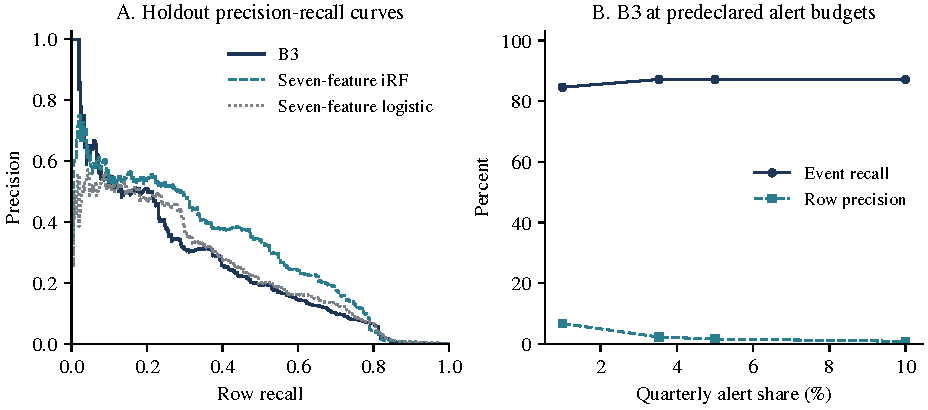
\includegraphics[width=\linewidth]{../figures/paper/holdout_ranking.pdf}
\caption{Holdout precision-recall curves and the B3 alert-share comparison.}
\label{fig:5}
\papernotes{Panel A uses all retained recall-change points. Panel B reports B3 at the predeclared alert shares. Sources: \evidence{pr_curve_display.csv} and \evidence{test_metrics.csv}.}
\end{figure}
\FloatBarrier
\subsection{Detection and review workload}
\begin{table}[!htbp]
\centering
\begin{threeparttable}
\caption{B3 confusion matrix at a quarterly alert share of 3.53\%.}
\label{tab:7}
\small\setstretch{1.0}\setlength{\tabcolsep}{4pt}\renewcommand{\arraystretch}{1.15}
\begin{tabular}{@{}L{\dimexpr 0.46656\linewidth-2\tabcolsep\relax}R{\dimexpr 0.17419\linewidth-2\tabcolsep\relax}R{\dimexpr 0.17419\linewidth-2\tabcolsep\relax}R{\dimexpr 0.18507\linewidth-2\tabcolsep\relax}@{}}
\toprule
\textbf{Observed outcome} & \textbf{No alert} & \textbf{Alert} & \textbf{Total} \\
\midrule
Failure within one year & 45 & 212 & 257 \\
No failure within one year & 264,296 & 9,310 & 273,606 \\
Total & 264,341 & 9,522 & 273,863 \\
\bottomrule
\end{tabular}
\begin{tablenotes}[flushleft]
\footnotesize\setstretch{1.0}
\item \textit{Notes.} The counting unit is a bank-quarter observation. Source: \evidence{test_metrics.csv}.
\end{tablenotes}
\end{threeparttable}
\end{table}
B3 detected 68 of 78 failures, giving event recall of 87.18\%. Of these, 49 failures were detected at least two quarters in advance. Across individual positive quarters, recall was 82.49\% and precision was 2.23\%. The confusion matrix contains 212 true positives and 9,310 false positives. Under the primary effort assumptions, these alerts required 23,004 review hours over the holdout, with a peak of 988 hours in one quarter.

The seven-feature iRF achieved higher mean annual AP than B3, at 0.310 versus 0.251. Logistic regression detected one additional failure at the same quarterly share. B3 remained the candidate selected during development. Its stronger development performance did not carry over to the holdout ranking, and the additional representation did not improve this final comparison.

\subsection{Spark MLlib demonstration}
The MLlib example fitted logistic regression using data through 2009 and evaluated it on 2011. The validation sample contained 29,834 rows, including 269 positives, and produced AP of 0.192 and ROC-AUC of 0.963. The pipeline included approximate-median imputation, vector assembly, scaling and regularization. Because these settings differ from the scikit-learn controls, this example evaluates the Spark modelling workflow separately from the principal model comparison.

\subsection{Model interpretation}
\begin{figure}[!htbp]
\centering
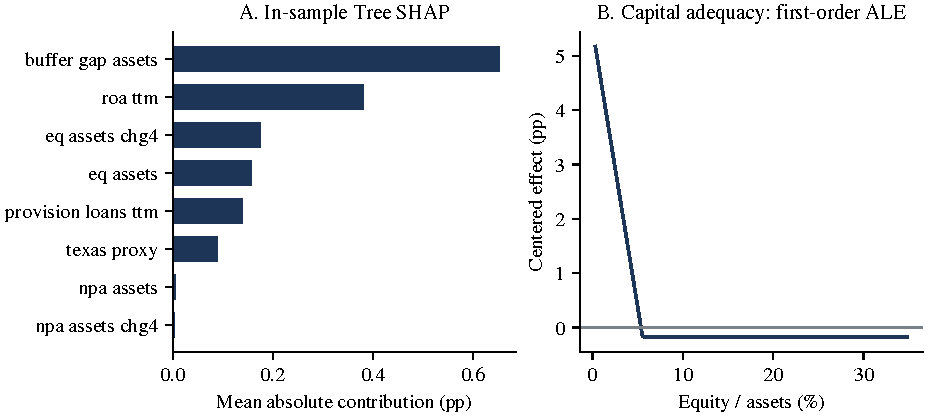
\includegraphics[width=\linewidth]{../figures/paper/explainability.pdf}
\caption{Development-sample explanations of B3.}
\label{fig:6}
\papernotes{Panel A reports mean absolute Tree SHAP contributions in percentage points for 96 uniformly sampled training observations. Panel B reports first-order ALE for equity/assets using 20,000 training observations. Sources: \evidence{final_B3_shap.csv} and \evidence{final_B3_ALE_eq_assets.csv}.}
\end{figure}
Path-dependent Tree SHAP was calculated from the fitted trees and the weighted number of training observations reaching each node \citep{treeshap}. Numerical checks compared the implementation with brute-force Shapley calculations on small examples and verified additivity for the fitted model. The attributions refer to the representation after clipping and median imputation.

Accumulated local effects (ALE) describe changes in model predictions within local feature intervals, which reduces reliance on the broad combinations of correlated inputs used in conventional partial-dependence plots \citep{ale}. Both explanations used development observations. Their role is to describe the fitted model, with correlated accounting measures potentially sharing attribution.

\section{Conclusions and implications for Vietnam}
\subsection{Storage, quality and early-warning performance}
The storage and processing results support a local columnar workflow for this panel. Retaining original response files preserved the acquisition record, while quarter-partitioned Parquet reduced storage and supported selective scans. Polars executed the matched transformation faster than pandas on the measured workload. Spark reproduced the calculations, although wider or concurrent workloads would be needed to assess a cluster advantage.

The main financial-data problems involved ambiguous zeros, missing histories, uncertain exits and changes in the basis of reported income. Exact calendar joins and records of reporting exceptions allowed these cases to receive distinct treatments before modelling. Historical data revisions and the assumed reporting lag remain limitations to evaluation using information available at the time. The rule isolating ambiguous historical thrift reports was also developed retrospectively. Together, these limitations prevent the evaluation from reproducing a dataset constructed solely from information available at each historical prediction date.

The holdout results support evaluating a review list through ranking and workload together. B3 detected most observed failures at the selected share but generated many false alerts, while the seven-feature iRF ranked the same holdout more accurately. Repeated development comparisons and the later addition of loss-buffer features may have favored the selected candidate \citep{cawley}. Since the holdout has now been evaluated, further model development would require a separate test window for an independent assessment.

Review costs remain a substantive empirical gap. Alert counts and review chains were measured from predictions, whereas unit effort and the weight on missed severity came from external proxies and scenario choices. Operational review logs would be needed to estimate those quantities and assess whether warnings change subsequent losses. The current cost results describe the specified decision scenarios.

\subsection{Adaptation to Vietnam}
An application in Vietnam would begin by mapping State Bank of Vietnam reporting definitions to the local balance-sheet and income fields, with institution identifiers linked through mergers and exits. Historical publication dates and revisions would be needed to reconstruct the information available at each prediction date. Distress outcomes would also need a local definition consistent with the intended supervisory action.

The review policy would then be estimated from local case-handling times, staff allocation and escalation records. Differences in funding structure and supervisory practice would require validation of the features and ranking model on Vietnamese institutions. The acquisition procedures, accounting checks and evaluation methods provide a starting point for that local validation.

\section{Reproducibility}
The accompanying code and executed notebook document the acquisition rules, financial transformations and evaluation procedure. The presentation notebook reads aggregate result tables, while separate commands reconstruct the private calculations from the documented data snapshot. Historical selector and model comparisons were retained with checksums identifying their source files. Final model fits, processing benchmarks and the holdout scoring were executed for this edition.

\begin{table}[!htbp]
\centering
\begin{threeparttable}
\caption{Materials provided with the project.}
\label{tab:8}
\small\setstretch{1.0}\setlength{\tabcolsep}{4pt}\renewcommand{\arraystretch}{1.15}
\begin{tabular}{@{}L{\dimexpr 0.30326\linewidth-2\tabcolsep\relax}L{\dimexpr 0.69674\linewidth-2\tabcolsep\relax}@{}}
\toprule
\textbf{Material} & \textbf{Contents} \\
\midrule
Executed notebook & Pipeline narrative and recorded outputs in 37 cells. \\
Source modules and tests & Acquisition, panel construction, features, metrics, review costs and numerical checks. \\
Aggregate tables and figures & Development comparisons, processing measurements, holdout results and sensitivity calculations. \\
Data and fitted models & Stored outside the public bundle, with acquisition and reconstruction instructions in the README. \\
Documentation & Source attribution, feature definitions, evaluation protocol and software requirements. \\
\bottomrule
\end{tabular}
\begin{tablenotes}[flushleft]
\footnotesize\setstretch{1.0}
\item \textit{Notes.} The selected modelling procedure has an extracted 64-fold replay implementation. Its full historical search was not rerun during preparation of this report. Documentation identifies the origin of inherited and newly computed results.
\end{tablenotes}
\end{threeparttable}
\end{table}
\FloatBarrier
The initial holdout population check stopped before prediction because its key list included unlabelled or ineligible records. Applying the existing label and population rules excluded 6,404 records from the 280,267 listed observations, leaving 273,863 eligible observations for evaluation. Model specifications and the alert share were unchanged during this correction. The execution record is retained with the evaluation protocol.

\FloatBarrier
\clearpage
\bibliographystyle{unsrtnat}
\bibliography{references}
\clearpage
\appendix
\label{appendix-start}
\section{Supplementary selector and model comparisons}
The following tables retain the stages of development in which selectors and model families were compared. Their experimental samples and selection rules are identified in the notes.

\subsection{Ranking and event detection}
\begin{table}[!htbp]
\centering
\begin{threeparttable}
\caption{Ranking and failure detection at the reference alert shares.}
\label{tab:9}
\small\setstretch{1.0}\setlength{\tabcolsep}{4pt}\renewcommand{\arraystretch}{1.15}
\begin{tabular}{@{}L{\dimexpr 0.30326\linewidth-2\tabcolsep\relax}R{\dimexpr 0.13935\linewidth-2\tabcolsep\relax}R{\dimexpr 0.18943\linewidth-2\tabcolsep\relax}R{\dimexpr 0.18943\linewidth-2\tabcolsep\relax}R{\dimexpr 0.17854\linewidth-2\tabcolsep\relax}@{}}
\toprule
\textbf{Model} & \textbf{Annual AP} & \textbf{Detected at 1\%} & \textbf{Detected at 5\%} & \textbf{Precision at 5\%} \\
\midrule
\addlinespace[3pt]\multicolumn{5}{@{}l}{\textit{Panel A. Fixed-origin validation}} \\
\addlinespace[2pt]
Seven-feature iRF & 0.220 & 399/514 & 481/514 & 5.27\% \\
Forward iRF & 0.243 & 387/514 & 477/514 & 5.41\% \\
Forward + T iRF & 0.248 & 376/514 & 481/514 & 5.49\% \\
\addlinespace[3pt]\multicolumn{5}{@{}l}{\textit{Panel B. Rolling-five-year validation}} \\
\addlinespace[2pt]
Seven-feature iRF & 0.198 & 335/514 & 484/514 & 5.08\% \\
Forward iRF & 0.207 & 341/514 & 482/514 & 5.26\% \\
Forward + T iRF & 0.213 & 343/514 & 488/514 & 5.47\% \\
\bottomrule
\end{tabular}
\begin{tablenotes}[flushleft]
\footnotesize\setstretch{1.0}
\item \textit{Notes.} Each scheme contains 594,873 rows, 1,981 positive rows and 514 failures. T denotes the four loss-buffer features. Source: \evidence{v65_branch_scores.csv}.
\end{tablenotes}
\end{threeparttable}
\end{table}
\subsection{Selector and model-family comparisons}
\begin{table}[!htbp]
\centering
\begin{threeparttable}
\caption{Eight leading candidates in the selector comparison.}
\label{tab:10}
\small\setstretch{1.0}\setlength{\tabcolsep}{4pt}\renewcommand{\arraystretch}{1.15}
\begin{tabular}{@{}L{\dimexpr 0.47744\linewidth-2\tabcolsep\relax}R{\dimexpr 0.17419\linewidth-2\tabcolsep\relax}R{\dimexpr 0.17419\linewidth-2\tabcolsep\relax}R{\dimexpr 0.17419\linewidth-2\tabcolsep\relax}@{}}
\toprule
\textbf{Selector and estimator} & \textbf{Fixed origin} & \textbf{Rolling 5y} & \textbf{Mean} \\
\midrule
mRMR + logistic & 0.235 & 0.182 & 0.209 \\
mRMR-HGB + logistic & 0.235 & 0.178 & 0.206 \\
Forward-HGB + logistic & 0.217 & 0.186 & 0.202 \\
Seven-feature logistic & 0.222 & 0.180 & 0.201 \\
L1 stability + logistic & 0.201 & 0.173 & 0.187 \\
Floating-HGB + logistic & 0.211 & 0.156 & 0.184 \\
Forward-HGB + HGB & 0.224 & 0.143 & 0.183 \\
Genetic-HGB + logistic & 0.200 & 0.160 & 0.180 \\
\bottomrule
\end{tabular}
\begin{tablenotes}[flushleft]
\footnotesize\setstretch{1.0}
\item \textit{Notes.} The mean averages the two scheme-specific annual AP values. mRMR denotes minimum redundancy maximum relevance, and HGB denotes histogram gradient boosting. Candidates were ordered by that mean. Original group-lasso estimates without established convergence were excluded. Source: \evidence{exp3d_fs1_d7.csv}.
\end{tablenotes}
\end{threeparttable}
\end{table}
\begin{table}[!htbp]
\centering
\begin{threeparttable}
\caption{Model families evaluated with the forward-selected representation.}
\label{tab:11}
\small\setstretch{1.0}\setlength{\tabcolsep}{4pt}\renewcommand{\arraystretch}{1.15}
\begin{tabular}{@{}L{\dimexpr 0.60808\linewidth-2\tabcolsep\relax}R{\dimexpr 0.19596\linewidth-2\tabcolsep\relax}R{\dimexpr 0.19596\linewidth-2\tabcolsep\relax}@{}}
\toprule
\textbf{Model} & \textbf{Fixed origin} & \textbf{Rolling 5y} \\
\midrule
Additive explainable boosting & 0.223 & 0.146 \\
Explainable boosting with pairwise terms & 0.225 & 0.143 \\
Histogram gradient boosting & 0.220 & 0.156 \\
Iterative random forest & 0.239 & 0.203 \\
Kernel approximation & 0.172 & 0.064 \\
Logistic regression & 0.198 & 0.185 \\
RuleFit & 0.202 & 0.164 \\
\bottomrule
\end{tabular}
\begin{tablenotes}[flushleft]
\footnotesize\setstretch{1.0}
\item \textit{Notes.} Training used all positives and a 20\% negative subsample without weighting. Scores are mean annual AP. The principal B3 comparisons used the full training sample. Source: \evidence{exp3d_fm1_d7.csv}.
\end{tablenotes}
\end{threeparttable}
\end{table}
\end{document}
